\documentclass[12pt,border=1pt]{standalone}
\usepackage[T1]{fontenc}
\IfFileExists{newtxtext.sty}{\usepackage{newtxtext,newtxmath}}{\usepackage{mathptmx}}
\usepackage{amsmath,amssymb}
\usepackage[table]{xcolor}
\usepackage{tikz}
\usetikzlibrary{arrows.meta,positioning,fit,calc,decorations.pathreplacing}
\tikzset{blk/.style={draw=black!55,rounded corners=2pt,align=center,font=\footnotesize,inner sep=4pt,minimum height=1.05cm},
         nn/.style={blk,fill=orange!12,draw=orange!70!black},
         lat/.style={blk,fill=blue!8,draw=blue!60!black},
         io/.style={blk,fill=black!3},
         arr/.style={-{Stealth[length=2.2mm]},thick,draw=black!65}}
\definecolor{capblue}{RGB}{47,84,150}
\definecolor{linkblue}{RGB}{17,85,204}
\definecolor{ganttA}{RGB}{11,90,110}
\definecolor{ganttB}{RGB}{20,150,160}
\definecolor{rowhl}{RGB}{253,236,224}
\definecolor{rowhl2}{RGB}{224,244,238}
\begin{document}
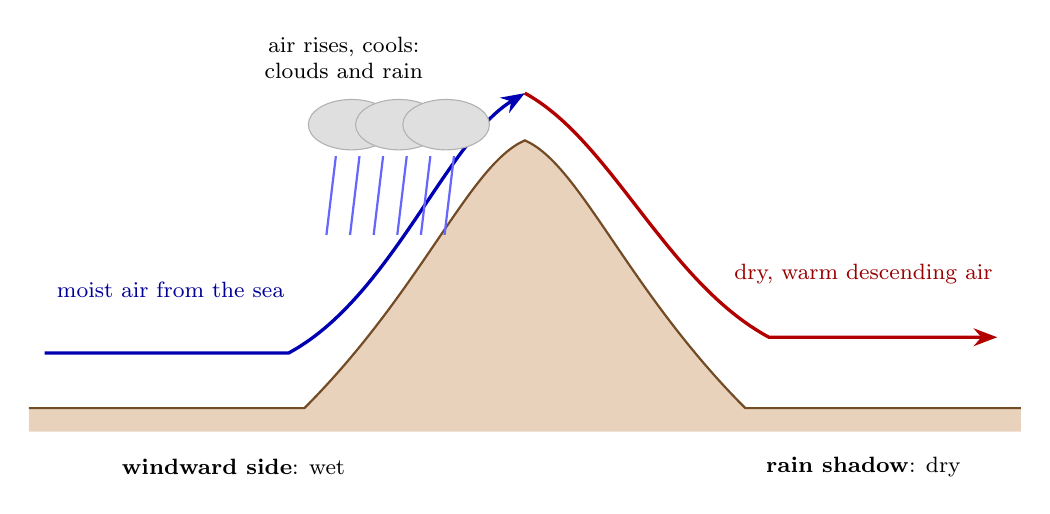
\begin{tikzpicture}[x=1cm,y=1cm]
\fill[brown!35] (0,0) -- (3.5,0) .. controls (5,1.5) and (5.6,3.1) .. (6.3,3.4) .. controls (7,3.1) and (7.6,1.5) .. (9.1,0) -- (12.6,0) -- (12.6,-0.3) -- (0,-0.3) -- cycle;
\draw[brown!60!black,thick] (0,0) -- (3.5,0) .. controls (5,1.5) and (5.6,3.1) .. (6.3,3.4) .. controls (7,3.1) and (7.6,1.5) .. (9.1,0) -- (12.6,0);
\draw[-{Stealth[length=3mm]},very thick,blue!70!black] (0.2,0.7) -- (3.3,0.7) .. controls (4.6,1.4) and (5.3,3.4) .. (6.3,4.0);
\draw[-{Stealth[length=3mm]},very thick,red!70!black] (6.3,4.0) .. controls (7.4,3.4) and (8.1,1.6) .. (9.4,0.9) -- (12.3,0.9);
\foreach \x in {4.1,4.7,5.3} \draw[fill=gray!25,draw=gray!60] (\x,3.6) ellipse (0.55 and 0.32);
\foreach \x in {3.9,4.2,4.5,4.8,5.1,5.4} \draw[blue!60,thick] (\x,3.2) -- (\x-0.12,2.2);
\node[font=\footnotesize,align=center,blue!60!black] at (1.8,1.5) {moist air from the sea};
\node[font=\footnotesize,align=center] at (4.0,4.45) {air rises, cools:\\clouds and rain};
\node[font=\footnotesize,align=center] at (2.6,-0.75) {\textbf{windward side}: wet};
\node[font=\footnotesize,align=center,red!60!black] at (10.6,1.7) {dry, warm descending air};
\node[font=\footnotesize,align=center] at (10.6,-0.75) {\textbf{rain shadow}: dry};
\end{tikzpicture}
\end{document}
